\documentclass[tikz,border=5pt]{standalone}

\usepackage{amsmath}
\usetikzlibrary{arrows.meta,calc,fit,positioning}

\definecolor{ink}{HTML}{17212B}
\definecolor{muted}{HTML}{5A6570}
\definecolor{panel}{HTML}{F7F8FA}
\definecolor{line}{HTML}{CED6DF}
\definecolor{street}{HTML}{0F766E}
\definecolor{remote}{HTML}{B45309}
\definecolor{crossview}{HTML}{7C3AED}
\definecolor{conflict}{HTML}{BE123C}
\definecolor{good}{HTML}{15803D}
\definecolor{softstreet}{HTML}{DDF4F0}
\definecolor{softremote}{HTML}{FCE7D2}
\definecolor{softcross}{HTML}{EEE7FF}
\definecolor{softconflict}{HTML}{FFE4E6}
\definecolor{softgood}{HTML}{DCFCE7}

\tikzset{
  panelbox/.style={
    draw=line,
    fill=panel,
    rounded corners=7pt,
    line width=0.55pt,
    minimum height=6.65cm
  },
  card/.style={
    draw=line,
    fill=white,
    rounded corners=5pt,
    line width=0.55pt
  },
  smallcard/.style={
    card,
    inner sep=4pt,
    align=center,
    font=\sffamily\scriptsize
  },
  tinylabel/.style={
    font=\sffamily\tiny,
    text=muted
  },
  paneltitle/.style={
    font=\sffamily\bfseries\small,
    text=ink,
    anchor=west
  },
  stepmark/.style={
    circle,
    fill=ink,
    text=white,
    font=\sffamily\bfseries\tiny,
    inner sep=1.6pt
  },
  flow/.style={
    -{Latex[length=2.2mm]},
    draw=ink,
    line width=0.75pt
  },
  softflow/.style={
    -{Latex[length=2mm]},
    draw=muted,
    line width=0.5pt
  },
  chip/.style={
    rounded corners=3pt,
    inner xsep=4pt,
    inner ysep=2.2pt,
    font=\sffamily\tiny\bfseries
  },
  formula/.style={
    card,
    fill=white,
    inner sep=5pt,
    align=center,
    font=\sffamily\scriptsize
  },
  metric/.style={
    card,
    inner sep=4pt,
    minimum width=2.35cm,
    align=center,
    font=\sffamily\scriptsize
  }
}

\begin{document}
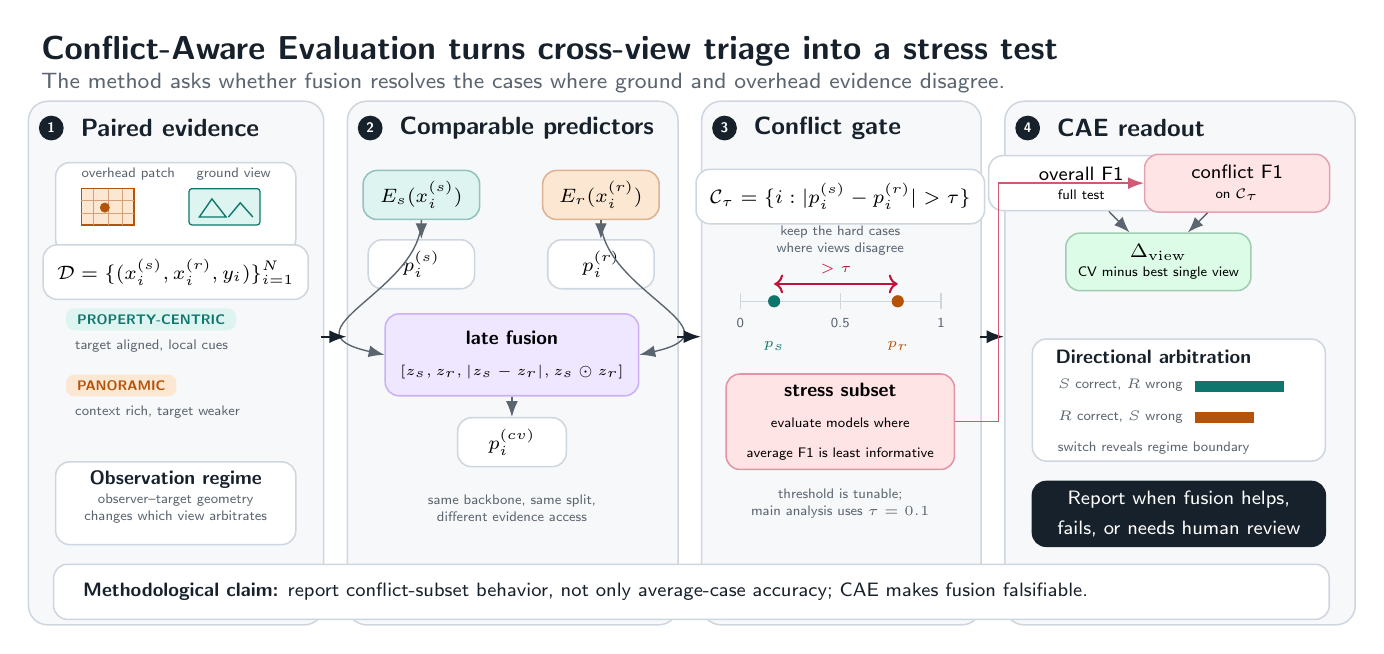
\begin{tikzpicture}[font=\sffamily, x=1cm, y=1cm]

% Panel frames.
\node[panelbox, minimum width=3.75cm, anchor=north west] (p1) at (0,0) {};
\node[panelbox, minimum width=4.20cm, anchor=north west] (p2) at (4.05,0) {};
\node[panelbox, minimum width=3.55cm, anchor=north west] (p3) at (8.55,0) {};
\node[panelbox, minimum width=4.45cm, anchor=north west] (p4) at (12.40,0) {};

% Global title.
\node[font=\sffamily\bfseries\large, text=ink, anchor=west] at (0.05,0.62)
  {Conflict-Aware Evaluation turns cross-view triage into a stress test};
\node[font=\sffamily\footnotesize, text=muted, anchor=west] at (0.05,0.22)
  {The method asks whether fusion resolves the cases where ground and overhead evidence disagree.};

% Panel titles.
\node[stepmark] at (0.30,-0.35) {1};
\node[paneltitle] at (0.55,-0.35) {Paired evidence};
\node[stepmark] at (4.35,-0.35) {2};
\node[paneltitle] at (4.60,-0.35) {Comparable predictors};
\node[stepmark] at (8.85,-0.35) {3};
\node[paneltitle] at (9.10,-0.35) {Conflict gate};
\node[stepmark] at (12.70,-0.35) {4};
\node[paneltitle] at (12.95,-0.35) {CAE readout};

% Panel 1: paired evidence and regimes.
\node[smallcard, minimum width=3.05cm, minimum height=1.15cm, anchor=north] (remoteCard) at (1.88,-0.78) {};
\node[tinylabel, anchor=west] at (0.56,-0.93) {overhead patch};
\draw[draw=remote, line width=0.45pt, fill=softremote] (0.68,-1.12) rectangle (1.35,-1.58);
\draw[draw=remote!55, line width=0.25pt] (0.84,-1.12) -- (0.84,-1.58)
  (1.02,-1.12) -- (1.02,-1.58)
  (1.20,-1.12) -- (1.20,-1.58)
  (0.68,-1.27) -- (1.35,-1.27)
  (0.68,-1.43) -- (1.35,-1.43);
\fill[remote] (0.98,-1.36) circle (1.8pt);
\draw[draw=street, line width=0.45pt, fill=softstreet, rounded corners=1pt] (2.05,-1.12) rectangle (2.95,-1.58);
\draw[street, line width=0.5pt] (2.18,-1.48) -- (2.34,-1.25) -- (2.52,-1.48) -- cycle;
\draw[street, line width=0.5pt] (2.55,-1.48) -- (2.70,-1.30) -- (2.86,-1.48);
\node[tinylabel, anchor=west] at (2.02,-0.93) {ground view};

\node[formula, minimum width=3.05cm] (dataset) at (1.88,-2.18)
  {$\mathcal{D}=\{(x_i^{(s)},x_i^{(r)},y_i)\}_{i=1}^{N}$};

\node[chip, fill=softstreet, text=street, anchor=west] at (0.48,-2.78)
  {PROPERTY-CENTRIC};
\node[tinylabel, anchor=west] at (0.48,-3.12)
  {target aligned, local cues};
\node[chip, fill=softremote, text=remote, anchor=west] at (0.48,-3.62)
  {PANORAMIC};
\node[tinylabel, anchor=west] at (0.48,-3.96)
  {context rich, target weaker};

\node[card, fill=white, minimum width=3.05cm, minimum height=1.05cm, anchor=north] at (1.88,-4.58) {};
\node[font=\sffamily\scriptsize\bfseries, text=ink] at (1.88,-4.82)
  {Observation regime};
\node[font=\sffamily\tiny, text=muted, align=center] at (1.88,-5.18)
  {observer--target geometry\\changes which view arbitrates};

% Panel 2: predictors.
\node[smallcard, fill=softstreet, draw=street!45, minimum width=1.48cm, minimum height=0.62cm] (Es) at (5.00,-1.20)
  {$E_s(x_i^{(s)})$};
\node[smallcard, fill=softremote, draw=remote!45, minimum width=1.48cm, minimum height=0.62cm] (Er) at (7.28,-1.20)
  {$E_r(x_i^{(r)})$};
\node[smallcard, fill=white, minimum width=1.35cm] (ps) at (5.00,-2.08)
  {$p_i^{(s)}$};
\node[smallcard, fill=white, minimum width=1.35cm] (pr) at (7.28,-2.08)
  {$p_i^{(r)}$};
\draw[softflow] (Es) -- (ps);
\draw[softflow] (Er) -- (pr);

\node[card, fill=softcross, draw=crossview!40, minimum width=3.22cm, minimum height=1.04cm, align=center] (fusion) at (6.15,-3.23)
  {\scriptsize\bfseries late fusion\\[-1pt]
   \tiny $[z_s,z_r,|z_s-z_r|,z_s\odot z_r]$};
\node[smallcard, fill=white, minimum width=1.38cm] (pcv) at (6.15,-4.34)
  {$p_i^{(cv)}$};
\draw[softflow] (Es.south) .. controls +(0,-0.90) and +(-1.35,0.30) .. (fusion.west);
\draw[softflow] (Er.south) .. controls +(0,-0.90) and +(1.35,0.30) .. (fusion.east);
\draw[softflow] (fusion) -- (pcv);
\node[tinylabel, align=center] at (6.15,-5.18)
  {same backbone, same split,\\different evidence access};

% Panel 3: conflict gate.
\node[formula, minimum width=2.90cm] (gate) at (10.32,-1.22)
  {$\mathcal{C}_{\tau}=\{i:|p_i^{(s)}-p_i^{(r)}|>\tau\}$};
\node[tinylabel, align=center] at (10.32,-1.78)
  {keep the hard cases\\where views disagree};

\draw[draw=line, line width=0.55pt] (9.05,-2.55) -- (11.60,-2.55);
\foreach \x/\lab in {9.05/0,10.32/0.5,11.60/1} {
  \draw[draw=line, line width=0.45pt] (\x,-2.45) -- (\x,-2.65);
  \node[tinylabel] at (\x,-2.83) {\lab};
}
\fill[street] (9.48,-2.55) circle (2.2pt);
\fill[remote] (11.05,-2.55) circle (2.2pt);
\draw[draw=conflict, line width=0.75pt, <->] (9.48,-2.33) -- node[above, font=\sffamily\tiny, text=conflict] {$>\tau$} (11.05,-2.33);
\node[tinylabel, text=street] at (9.48,-3.12) {$p_s$};
\node[tinylabel, text=remote] at (11.05,-3.12) {$p_r$};

\node[card, fill=softconflict, draw=conflict!45, minimum width=2.90cm, minimum height=1.18cm, align=center] (stress) at (10.32,-4.08)
  {\scriptsize\bfseries stress subset\\[-1pt]
   \tiny evaluate models where\\[-1pt]
   \tiny average F1 is least informative};
\node[tinylabel, align=center] at (10.32,-5.12)
  {threshold is tunable;\\main analysis uses $\tau=0.1$};

% Panel 4: CAE readout.
\node[metric, fill=white] (m1) at (13.38,-1.05)
  {overall F1\\[-1pt]\tiny full test};
\node[metric, fill=softconflict, draw=conflict!40] (m2) at (15.36,-1.05)
  {conflict F1\\[-1pt]\tiny on $\mathcal{C}_{\tau}$};
\node[metric, fill=softgood, draw=good!40] (m3) at (14.36,-2.05)
  {$\Delta_{\mathrm{view}}$\\[-1pt]\tiny CV minus best single view};
\draw[softflow] (m1) -- (m3);
\draw[softflow] (m2) -- (m3);

\node[card, fill=white, minimum width=3.72cm, minimum height=1.55cm, anchor=north] (bars) at (14.62,-3.02) {};
\node[font=\sffamily\scriptsize\bfseries, text=ink, anchor=west] at (12.93,-3.25)
  {Directional arbitration};
\node[tinylabel, anchor=west] at (12.96,-3.62) {$S$ correct, $R$ wrong};
\draw[fill=street, draw=none] (14.82,-3.70) rectangle (15.96,-3.56);
\node[tinylabel, anchor=west] at (12.96,-4.02) {$R$ correct, $S$ wrong};
\draw[fill=remote, draw=none] (14.82,-4.10) rectangle (15.58,-3.96);
\node[tinylabel, anchor=west] at (12.96,-4.42) {switch reveals regime boundary};

\node[card, fill=ink, draw=ink, minimum width=3.72cm, minimum height=0.82cm, align=center] at (14.62,-5.25)
  {\color{white}\scriptsize Report when fusion helps,\\[-1pt]
   \color{white}\scriptsize fails, or needs human review};

% Inter-panel arrows.
\draw[flow] (3.72,-3.00) -- (4.05,-3.00);
\draw[flow] (8.25,-3.00) -- (8.55,-3.00);
\draw[flow] (12.10,-3.00) -- (12.40,-3.00);

% Keep cross-panel flow sparse so the figure reads as an argument, not a wiring diagram.
\draw[softflow, draw=conflict!70] (stress.east) -- +(0.55,0) |- (m2.west);

% Bottom claim strip.
\node[card, fill=white, draw=line, minimum width=16.20cm, minimum height=0.70cm, anchor=west] at (0.32,-6.24) {};
\node[font=\sffamily\scriptsize, text=ink, anchor=west] at (0.58,-6.24)
  {\textbf{Methodological claim:} report conflict-subset behavior, not only average-case accuracy; CAE makes fusion falsifiable.};

\end{tikzpicture}
\end{document}
